% Background Information

\chapter{Background Information} % Main chapter title

\label{chap:Background} % For referencing the chapter elsewhere, use \ref{Background} 


%----------------------------------------------------------------------------------------

\section{Graph}
	\subsection{Definition}
	A graph is defined as a structure with a set of nodes called vertices ($V$) and a set of links between these nodes called edges ($E$). By this definition a graph ($G$) becomes a two-element tuple of the following form.
	\begin{equation} G = (V, E) \end{equation}	
	Traversing a graph from some vertex $v1$ to some $v2$ along the edge $(v1, v2)$ is written as:
	\begin{equation} v1 \stackrel{(v1, v2)}{\to} v2 \end{equation}
	A path with an arbitrary number of edge-traversals leading from $v1$ to $v2$ is written as:
	\begin{equation} v1 \to^* v2 \end{equation}
	
	\subsection{Strongly Connected Components}
	A directed graph is said to be \emph{strongly connected} if every vertex $v \in V$ is reachable from any other vertex $v2 \in V$. Here $v1$ and $v2$ can be the same vertex.
	\begin{equation}v1, v2 \in V : \prodstar{v1}{v2}\end{equation}
	The set of \emph{\textbf{strongly connected components}} of a directed graph $G$ is defined as the partitioning of $G$ into smaller graphs, such that all of these subgraphs are strongly connected.
	\begin{figure}[h]
		\centering
		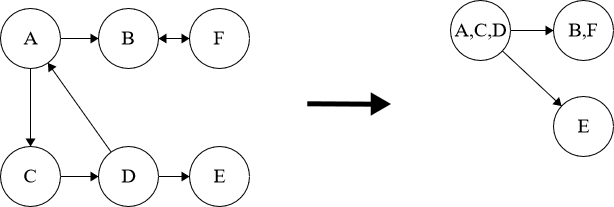
\includegraphics[scale=0.6]{Figures/components.png}
		\decoRule
	 	\caption[Strongly connected components]{The strongly connected components of a graph}
	 	\label{fig:GraphExample}
	\end{figure}
	
		\subsubsection{Kosaraju's algorithm}
		\label{sec:Kosaraju}
		Numerous algorithms for computing the strongly connected components of a directed graph exist. Most of these also have nice time-complexities. Kosaraju's algorithm works in $\mathcal{O}(V+E)$. Officially published by \parencite{Kosaraju}, it uses the property of the inverse of a directed graph having the same strongly connected components as the original graph. Below follows a brief description of the algorithm. A few things beforehand:
		
		\begin{enumerate}
			\item A component is represented by assigning every vertex a root vertex of its component.
			\item The algorithm requires an ordered list $L$ of vertices. It will grow to contain each vertex once.
		\end{enumerate}
		The algorithm then becomes:
		\begin{enumerate}
			\item For each vertex $u \in V$, mark $u$ as unvisited. let $L$ be empty.
			\item For every vertex $u \in V$ $Visit(u)$, where $Visit(u)$ is:
				\subitem if $u$ is unvisited:
					\subsubitem Mark $u$ as visited
					\subsubitem For each out-neighbour $v$ of $u$, $Visit(v)$
					\subsubitem Prepend $u$ to $L$
			\item For each element $u$ in $L$ (in order), $Assign(u,u)$, where $Assign(u,root)$ is:
				\subitem If $u$ has not been assigned to a component:
					\subsubitem Assign $u$ as beloging to the component whose root is $root$
					\subsubitem For each in-neighbour $v$ of $u$, do $Assign(v, root)$
		\end{enumerate}
		
		
		
	\pagebreak
	
\section{Context-Free Grammar}
	\subsection{Definition}	\label{sec:CFG_def}
	A context-free grammar ($CFG$) is a 4-element tuple. It has two disjoint alphabets $V$ and $\Sigma$, a set of production rules $P$ and a startsymbol $S \in V$. A production rule $p$ is a pair $(A, w)$ with $A \in V$ and $w \in (V \cup \Sigma)^*$. The set $\Sigma$ is the set of terminals and $V$ the set of non-terminals. Empty sentences are defined by $\epsilon$\\
	\begin{equation} CFG = (V, \Sigma, P, S) \end{equation}	
	\begin{equation} p \in P, A \in V, A \rightarrow w \in (V \cup \Sigma)^*\end{equation}	
			
	\subsection{Graph of a CFG} \label{eqn:gram2graph}
	The graph of a context-free grammar is defined as follows. It is a directed graph with vertices for each non-terminal in $CFG$ and an edge from a non-terminal $A \in V$ to some other $B \in V$ iff $B$ is in $w$ for some production rule $A \rightarrow w$.
	\begin{align} 
	\vspace{-0.3in}
	\nonumber CFG &= (V_{cfg}, \Sigma, P, S)\\
	\vspace{0.1in}
	\nonumber E &= \{(A, B) | (A \rightarrow w) \in P, B \in w, B \in V_{cfg}\}\\
	\vspace{0.1in}
	G &= (V_{cfg}, E)
	\end{align}
		
	\subsection{Strongly Regular Grammars}
	\label{sec:MohriNederhof}
	Normal context-free grammars can generate languages that are not regular. In other words, these can not be mapped to equivalent finite state machines. The subclass of grammar called \emph{strongly regular grammars} are the set of grammars guaranteed to generate regular languages. This set is also the set of grammar without self-embedding \parencite{Chomsky1959}.\\\\
	Strongly regular grammars are grammars in which the rules of each set $M$ of mutually recursive nonterminals are either all right-linear or all left-linear. All non-terminals $T \not \in M$ are considered terminals here. For the sake of this thesis I chose to use the case of right-linear grammars and rewrite all conflicting rules to right-linear ones. \cite{MohriNederhof} describe a simple transformation to transform any grammar into a strongly regular one. The new grammar accepts a superset of the language of the original grammar.
	\pagebreak
	\begin{enumerate}
		\item Identify all sets $M$ of \textit{mutually recursive non-terminals}\footnote{This coincides with the strongly connected components of the grammar} such that not all\\ $p:(\prodgr{A}{w}), A \in M$ are right- or left-linear with respect to other elements of $M$.
		\item For all non-terminals with conflicting productions $A \in M, p:(\prodgr{A}{w})$ introduce a new non-terminal $A' \not \in V$. 
		\item If $A$ is directly reachable from some other non-terminal $X \not \in M$ introduce a rule $\prodeps{A'}$.
		\item For all rules with left hand side $A \in M$:
		\subitem $\prodgr{A}{\alpha_0 B_1 \alpha_1 B_2 \dots \alpha_m B_m}\vspace{0.1in}$\\
		with $m \geq 0, B_1, \dots, B_m \in M, \alpha_0, \ldots, \alpha_m \in (\Sigma \cup (N - M))^*$. Replace with:
		\begin{align}
		\nonumber \alprod{A}{\alpha_0 B_1}
		\\\nonumber \alprod{B'_1}{\alpha_1 B_2}
		\\\nonumber \alprod{B'_2}{\alpha_2 B_3}
		\\\nonumber &\ldots
		\\\nonumber \alprod{B'_{m-1}}{\alpha_{m-1} B_m}
		\\\nonumber \alprod{B'_m}{\alpha_m A'}
		\end{align}
		\item if $m = 0$, we end up with just $\prodgr{A}{\alpha_0 A'}$.					
	\end{enumerate}
	This transformation ensures that all rules of the grammar become right- or left-linear with respect to their set of recursively reachable symbols. This ensures a regular grammar and therefore that it is possible to convert this new grammar into state machines

\pagebreak

\section{State Machines}
	\subsection{Definition}
		A deterministic finite state machine (DFSM or DFA) $S$ is a 5-element tuple with a set of states ($Q$), an alphabet ($\Sigma$), an initial state ($q_0 \in Q$), a set of final states ($F \subseteq Q$) and a transition function ($\delta : (Q \times \Sigma \rightarrow Q)$) describing how to move from one state to the next. Alongside this we define a transition as a 3-element tuple.
		\begin{equation} S = (Q, \Sigma, q_0, F, \delta) \end{equation}
		\begin{equation} Tr = (q_1, a \in \Sigma, q_2) \end{equation}
		For a non-deterministic variant (NFSM or NFA) we make 2 small changes. 
		\begin{enumerate}
			\item $\epsilon$ is allowed as an element of $\Sigma$. This was not allowed for a DFA.
			\item $\delta$ becomes a function to the power set of $Q$: $(Q \times \Sigma) \rightarrow \mathbb{P}(Q)$)
		\end{enumerate}
			
	\subsection{Machines for Strongly Regular Grammars}	\label{sec:ComponentMachine}
	You can construct finite automata for strongly regular grammars. You can either generate one (potentially enormous) machine, or go with a more compact representation. The general steps of the algorithm for this compact version can be sketched as follows:
	\begin{enumerate}
		\item Determine the sets of mutually recursive non-terminals. 
		\item For each set $M$ create one machine $\mathcal{K}(M)$ using the classical construction of an automaton from a grammar. $\mathcal{K}(M)$ is now an NFA for which we have left the starting state unspecified. Here are all non-terminals that are not part of $M$ seen as terminals and put on transition-arcs. 
		\item To obtain a machine that accepts string generated by some non-terminal $A$ we just pick the machine $\mathcal{K}(M)$ for which $A \in M$. Now we choose the state corresponding to $A$ as the starting state ($q_A$). This is the machine accepting the language of $A$.
		\item To accept the entire language find the following machine:
		\subitem \begin{equation*}\mathcal{N}(S) = \mathcal{K}(M) , S \in M , (q_0 = q_S \in Q)\end{equation*}
		Now while processing input strings $w$ we lazily substitute new machines into $\mathcal{N}(S)$ once we encounter non-terminals outside $M : S \in M$.
	\end{enumerate}
	
\pagebreak

\section{State-Based Syntax Highlighters}
	\subsection{Definition}
	Different editors tend to use different formats for state-based highlighters. Although much of the structure and elements are similar. This thesis is focused on working with Sublime Text as a first try. This was chosen for convenience of availability and clarity of a so-called \file{.sublime-syntax} file.\\\\
	A state-based syntax highlighter is basically a simple automaton. It has states, sentences determining where to go next and a starting state (\emph{main}). There is the addition of a stack to the machine. This stack is for keeping track of which state(s) the highlighter is in. Transitioning from one state to another, means replacing the current state with the next state on the stack. This operation is called \emph{set}. Besides this action we have three additional options. \textit{1.} \emph{push} the next state on the stack, \textit{2.} \emph{pop} the current state off of the stack, \textit{3.} push or set a list of states. This last one means simply pushing a list of contexts, or for the \textit{set}-action it means replacing and pushing. Sadly there is no pop $n$ states from the stack.\\
	The states of this 'state machine' are called \emph{contexts}. These are state like structures which \emph{match} a number of regular expressions. These cause action (like changing context or colouring the match). The type we assign to our matches are called \emph{scopes}. This is a highlighting scope. These are predefined and help all editors and different colouring themes to still produce correct results with the same highlighter. The combination of a regular expression and assigning contexts or scopes are appropriately called \emph{matches}. \emph{Variables} are predefined regular expressions that can be reused throughout different contexts.\\\\
	In formal terms this becomes, where yet to be defined terms will be explained in the rest of this section:
	\begin{align} \label{eqn:highlighterDef}
	  \nonumber Highlighter &= H
	\\\nonumber Contexts   	&= C
	\\\nonumber Matches 	&= M
	\\\nonumber Scopes  	&= S
	\\\nonumber Variables  	&= V
	\\\nonumber Actions  	&= A
	\\\nonumber main &\in C
	\\\nonumber H &= (name,\ file\_extensions,\ V,\ C,\ main)
	\\\nonumber (c \in C) \Rightarrow c &= (M' \subseteq M,\ \ s \in S)
	\\\nonumber (s \in S) \Rightarrow s &\in (meta\_scope(scope\_name),\ scope(scope\_name),\ null())
	\\\nonumber (m \in M) \Rightarrow s &= (regex, s \in S, a \in A)
	\\\nonumber (a \in A) \Rightarrow a &\in \{set(S' \subseteq S),\ push(S' \subseteq S),\ pop(),\ noact()\}
	\end{align}
	Below are the namings and actions of two editors and their syntax-definitions shown. They both show an example of a highlighter producing equivalent results. The just defined names are closely related to how Sublime text works, because that has been the main editor used in this project. Therefore the highlighter information on TextMate is also more bare.


	\subsection{The TextMate JSON-like Syntax Definition}
	In TextMate\footnote{source: \cite{website:TextmateSyntax}} you make use of a $JSON$-like definition as seen below. This highlighter highlights two things. The words \verb|'for', 'while', 'return', 'if'| are highlighted as keywords. And everything from an opening double-quote up till the corresponding closing one is highlighted as if it were a string. Except for characters that are escaped by a backslash. These get a special colouring for constants.\\
	As can be observed below contexts are named patterns for TextMate. They have either simple matches, with a scope assigned to $name$ or a 'begin' and 'end' match. This corresponds to: match 'begin' $\rightarrow$ push nested 'patterns' (contexts) on the stack. Then on matching the 'end' you pop de nested context(s) off of the stack. The actual presence of the stack is more concealed for TextMate. For these second type of matches, if the match has a scope specified, all characters that are passed whilst being in this context will be highlighted with that scope (including the begin and end matches, however this is adjustable).
	\subsubsection{A TextMate highlighter}
	\lstinputlisting[style=highlighter, caption={A TextMate example highlighter}, language=Python]{Code/highlighters/textMate_example.syntax}
	\pagebreak
	
	\subsection{The Sublime YAML-like Syntax Definition} \label{sec:SublimeSyntax}
	As seen in the files below there are some differences between Sublime\footnote{source: \cite{website:SublimeSyntax}} and TextMate. However they also have a lot in common. The biggest difference may be that Sublime does not have the nice 'begin' and 'end' matches which make multiline matches much easier. In Sublime you have to do this yourself. This can cause problem when working with multiline portions like comments. Beside that, the starting context is always named "main"\\
	A few more things can be done with the Sublime highlighters (many of these are also available in some form in TextMate). First of all the "- include:" statements. These statements allow to be in multiple contexts at a time. It can be seen as a union of this context with the included one. The formal definitions of the highlighter $H$ and contexts $C$ could be extended by adding a set of $incudes$ to the tuple. Secondly, just like with TextMate you can nest contexts and make them nameless. Finally there is the concept of the $prototype$ scope. This is a scope that is always included in every other scope (unless specified otherwise). This is useful in for example highlighting comments, these can occur nearly everywhere. This could also be added to  the definition of $H$.\\
	Just like TextMate you can have everything that is encountered whilst being in a context highlighted with the same colouring. This is done through assigning a so-called meta-scope to the context.
	
		\subsubsection{Line endings} \label{sec:SublimeSyntax:LineEndings}
		In Sublime the regular expressions are always matched against a single line. This can cause trouble in a number of situations. Imagine having a context that processes whitespace without doing anything with it. It should pop itself off of the stack once there is no more whitespace:
		\begin{lstlisting}[language=Python]
		Whitespace:
			- match: '[\n\t\ \f\r]'
			- match: '?!([\n\t\ \f\r])'
			  pop: true
		\end{lstlisting}	
		This seems to be fine. It keeps matching whitespace until it no longer matches whitespace (using lookahead so it does not consume the matched character). Then pops itself of. However in the code below this will produce unexpected results. after the opening '\{' it will find and parse the space and newline, match these and do nothing. Now the following characters will be a tab, however the highlighter is now right before the line-ending (\$). This will fail the first match and pass the second match, since it matches not whitespace following the caret, and pop off the context. This type of behaviour should be taken into account. 
		\begin{lstlisting}[language=Java]
		if (condition) { 
			Statement;
		}
		\end{lstlisting}
		\pagebreak	
		
	\subsubsection{A Sublime highlighter}
	\lstinputlisting[language=SublimeSyntax, caption={A Sublime example highlighter}]{Code/highlighters/sublime_example.sublime-syntax}